a)
\begin{figure}[H]
    \centering
    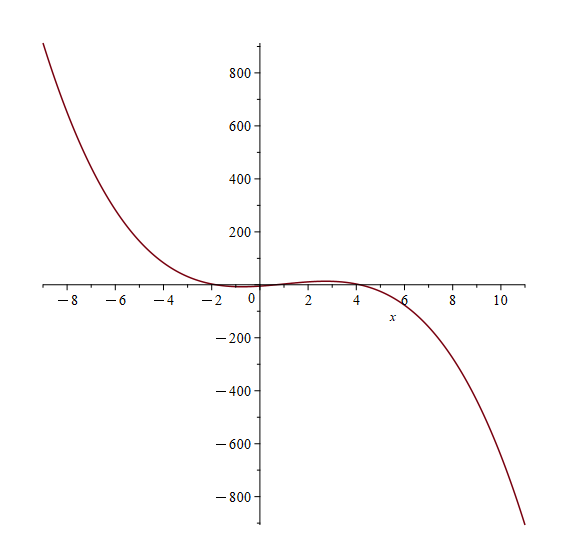
\includegraphics[width=1\linewidth]{Billeder/6.png}
\end{figure}

b)
Jeg kan bestemme monotoniforholdene ved at sætte den differentierede til nul. Så får jeg alle de lokale maximum- og minimumsværdier. Her bruger jeg igen solve-funktionen fra Maple:
$$f'(x)=0, x=1-\sqrt{3} \quad\cap\quad 1 + \sqrt{3}$$
Grafen er altså faldene fra $]-\infty;1-\sqrt{3}[$, stigende i $]1-\sqrt{3};1 + \sqrt{3}[$ og igen faldende i $]1 + \sqrt{3};\infty[$.\newline

c)
Den differentierede angiver en hældning af stamfunktionen, derfor kan jeg sætte $f'(x)$ lig med 9 og dermed finde det punkt, hvor tangenten ligger.
Igen ved hjælp af Maples' solve-funktion:
$$f'(x)=9, x=1$$
Altså er førstekoordinaten til røringspunktet for tangenten $1$.\newpage